% Desenvolvido para o IFSP por: Prof. Dr. David Buzatto (Versão 1.0.2, Data: 31/01/2023)
% Acessado em <https://github.com/davidbuzatto/TemplatesTrabalhosIFSPSBV/tree/master/Template%20Latex%20-%20Apresentacao%20-%20IFSP%20-%20SBV> em 02/02/2023
% Licença Creative Commons CC BY 4.0
% Adaptado para a UFMG por: Dra. Cecilia F. Fiorini (Data: 02/02/2023)

\documentclass[aspectratio=169]{beamer}
% a opção hideSubsectionTitle esconde o título das subseções
\usepackage{estruturaApresentacao}
\usepackage[alf,abnt-emphasize=bf]{abntex2cite}

\begin{document}

\titulo{Otimização do gasto energético em um galpão de bobinas quentes de aço}
% caso não haja, comente a linha abaixo
\subtitulo{Uma abordagem de programação linear}

\autor{Everson Elias \& Josoe S. Queiroz \& Valentim Neto \& Victor Hugo}
% % caso não haja, comente a linha abaixo
% \coorientador{Prof./Profa. Me./Dr./Dra. Nome Completo}

\curso{Engenharia de sistemas}

% exemplos
%\curso{Bacharelado em Ciência da Computação}
%\curso{Tecnologia em Sistemas para Internet}
%\curso{Especialização em Desenvolvimento de Aplicações para Dispositivos Móveis}

\local{Belo Horizonte}
\dia{04}
\mes{06}
\ano{2025}


% não mexa!

\begin{frame}[plain]
    
    \begin{tikzpicture}[overlay,remember picture]
        \node[left=-0.15cm] at (current page.0){
            
\includegraphics[scale=0.202]{imagens/capa}
        };
    \end{tikzpicture}
    
    \titlepage
    
\end{frame}

\section[Agenda]{}

\begin{frame}
    \frametitle{Agenda}
    \tableofcontents
\end{frame}
\section{Introdução}

\begin{frame}

    \frametitle{Introdução - Motivação}
    % neste frame vamos ter que falar que há a oportunidade de reduzir gasto energético em outras partes da produção onde não se gasta energia para esquentar o metal.
    \begin{itemize}
        % \item Aço é essencial para muitas indústrias
        \item Em 2023, estima-se que foram produzidas 1,9 bilhão de toneladas de aço no mundo. \cite{worldsteel.org_2024}
        \item Todas as etapas do processo produtivo de ação são extremamente intensas em gasto energético. O custo de produção de todo esse metal é de aproximadamente 20.99 GJ/ton o que resulta em $39,88\times10^{15}J (Peta)$ no total.
        \item Reduzir o custo energético da produção de metais é essencial para o crescimento sustentável da sociedade global.
    \end{itemize}
\end{frame}

% \begin{frame}{Introdução - Produção de aço}
%     \begin{figure}
%         \centering
%         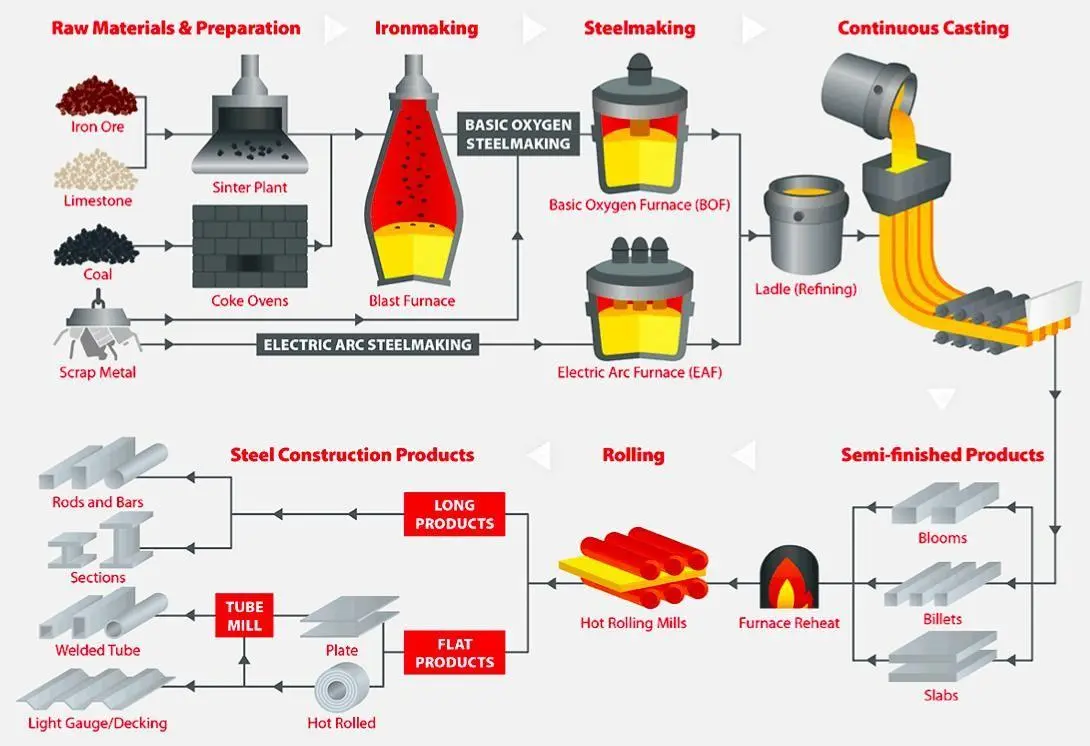
\includegraphics[width=0.55\linewidth]{imagens/ciclo_producao_aco.png}
%         \caption{Ciclo de produção do Aço}
%         \label{fig:ciclo-producao-aco}
%     \end{figure}
% \end{frame}
% \begin{frame}{Introdução - Produção de aço}
%     \begin{figure}
%         \centering
%         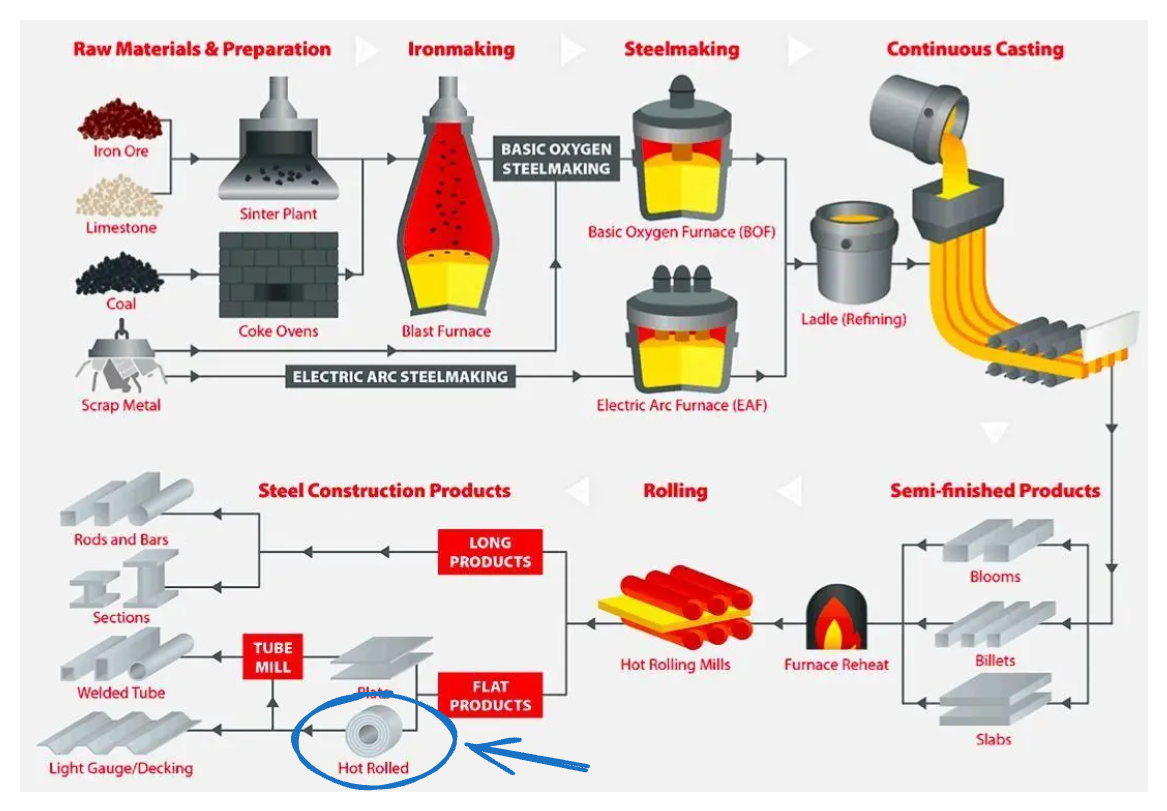
\includegraphics[width=0.55\linewidth]{imagens/ciclo-producao-aco-1.png}
%         \caption{Ciclo de produção do Aço}
%         \label{fig:ciclo-producao-aco-1}
%     \end{figure}
% \end{frame}

\begin{frame}{Introdução - Armazenamento de bobinas quentes}
    \begin{figure}
        \begin{figure}
            \centering
            \includegraphics[width=0.5\linewidth]{imagens/rolled-coils-in-storage.png}
            \caption{Bobinas diferentes em armazenamento}
            \label{fig:bobinas-armazenamento}
        \end{figure}
    \end{figure}
\end{frame}
\begin{frame}

    \frametitle{Introdução - Objetivos}

    \begin{itemize}
        %\item Buscar reduzir o custo de operações que não envolvem o tratamento do metal quente
        \item Organizar as bobinas em um depósito de forma a minimizar os movimentos futuros e, consequentemente, os gastos energéticos, visando a uma distribuição (\textit{layout}) ótima para atender às demandas previstas.
        \begin{itemize}
            %\item Focar na otimização da organização de bobinas quentes armazenadas
            %\item Simplificar a o planejamento diário dos armazéns
            \item Assumimos que conhecemos com antecedência as demandas que devem ser atendidas.
            \item Assumimos plena disponibilidade de maquinário e de pessoal para realizar as movimentações necessárias.
        \end{itemize}
    \end{itemize}
\end{frame}

% exemplos de construções em LaTeX
% comente a linha abaixo para gerar a versão final


\section{Descrição do Problema}

\begin{frame}{Descrição do Problema - Notação e Variáveis do Modelo}
\textbf{Variáveis de Decisão:}
\begin{itemize}
    \item $W^s_{kq,a}$: Ponte rolante \textbf{carregada} move a bobina $a$ da posição $k$ para $q$ na seção $s$.
    \item $V^s_{kq}$: Ponte rolante \textbf{vazia} se move da posição $k$ para $q$ na seção $s$.
    \item $x^s_{q,a}$: Bobina $a$ está armazenada na posição $q$ durante a seção $s$.
    \item $\tau_s \in \mathbb{R}$: Tempo de início da seção $s$.
\end{itemize}

\vspace{0.4cm}
\textbf{Outras Notações:}
\begin{itemize}
    \item $\Phi$: Conjunto de posições válidas no galpão.
    \item $\Psi$: Conjunto de posições disponíveis para armazenamento (nível 1 e 2).
    \item $A_{in}, A_{out}$: Conjuntos de bobinas a serem armazenadas ou retiradas.
    \item $t^{\text{load}}_{kq},\ t^{\text{empty}}_{kq}$: Tempo para movimentações carregadas e vazias.
    \item $E^{\text{load}}_{kq},\ E^{\text{empty}}_{kq}$: Energia consumida em cada tipo de movimentação.
\end{itemize}
\end{frame}

%%%%%%%%%%%%%%%%%%%%%%%%%%%%%%%%%%%%%%%%%%%%%%%%%%%%%%%%%%%%%%%%%%%%%%%%%%%%%%%%%%%%%%%%%%%%%%%%%%%%%%%%%%%%%%%%%%

\begin{frame}{Descrição do Problema - Função Objetivo}
\textbf{Objetivo:} Minimizar o consumo total de energia das movimentações da ponte rolante (carregadas e vazias).

\vspace{0.3cm}

\begin{block}{Função Objetivo:}
    \[
    \min E = 
    \sum_{k \in \Phi} \sum_{q \in \Phi} \sum_{s \in S} \sum_{a \in A} 
    \left( E^{\text{load}}_{kq,a} \cdot W^s_{kq,a} \right) +
    \sum_{k \in \Phi} \sum_{q \in \Phi} \sum_{s \in S}
    \left( E^{\text{empty}}_{kq} \cdot V^s_{kq} \right)
    \]
\end{block}

\vspace{0.4cm}
\textbf{Significado:}
\begin{itemize}
    \item Primeiro termo: custo energético de movimentações \textbf{carregadas}.
    \item Segundo termo: custo energético de movimentações \textbf{vazias}.
    \item O modelo busca um \textbf{planejamento ótimo} que minimize o total de energia consumida.
\end{itemize}
\end{frame}

%%%%%%%%%%%%%%%%%%%%%%%%%%%%%%%%%%%%%%%%%%%%%%%%%%%%%%%%%%%%%%%%%%%%%%%%%%%%%%%%%%%%%%%%%%%%%%%%%%%%%%%%%%%%%%%%%%%%

\begin{frame}{Descrição do Problema - Principais Restrições}
\textbf{Para modelagem, tivemos 18 restrições. As restrições foram agrupadas em 4 categorias:}
\begin{itemize}
    \item \textbf{1. Entrada e Saída:} garantem que todas as bobinas entrem ou saiam corretamente.
    \item \textbf{2. Ocupação e Capacidade:} cada bobina ocupa apenas um espaço, e cada espaço só pode conter uma bobina.
    \item \textbf{3. Precedência Temporal:} movimentações só ocorrem após a anterior ser finalizada.
    \item \textbf{4. Empilhamento e Bloqueios:} respeitam as regras de empilhamento entre níveis (bloqueios superiores/inferiores).
\end{itemize}

\end{frame}

%%%%%%%%%%%%%%%%%%%%%%%%%%%%%%%%%%%%%%%%%%%%%%%%%%%%%%%%%%%%%%%%%%%%%%%%%%%%%%%%%%%%%%%%%%%%%%%%%%%%%%%%%%%%%%%%%%%%

\begin{frame}{Exemplos de Restrições por Categoria}

\begin{block}{1. Entrada e Saída:}
  \[
    \sum_{q \in \Phi \,|\, q \ne I} \sum_{s \in S} W^s_{Iq,a} = 1 \quad \forall a \in A_{in}
    \]
    \textit{Cada bobina que entra deve ser movimentada a partir da posição de entrada.}
\end{block}

\vspace{0.2cm}
\begin{block}{2. Ocupação e Capacidade:}
    \[
    \sum_{k \in \Phi} x^s_{ka} = 1 \quad \forall a \in A,\ s \in S
    \]
    \textit{Cada bobina ocupa uma única posição por seção.}
\end{block}

\vspace{0.2cm}

\end{frame}

\begin{frame}{Exemplos de Restrições por Categoria}
\begin{block}{3. Precedência Temporal:}
   \[
    \tau_s \geq \tau_{s-1} +
    \sum_{k \in \Phi} \sum_{q \in \Phi} \left( t^{empty}_{kq} \cdot V^{s-1}_{kq} \right)
    +
    \sum_{k \in \Phi} \sum_{q \in \Phi} \sum_{a \in A} \left( t^{load}_{kq} \cdot W^{s-1}_{kq,a} \right)
    \quad \forall s \in S,\ s \ne 1
    \]
    \textit{As ações da seção atual só podem iniciar após o fim das ações da seção anterior.}
\end{block}

\vspace{0.2cm}
\begin{block}{4. Empilhamento e Bloqueios:}
    \[
    \sum_{q \in \Phi} \sum_{a \in A} W^s_{kq,a} \leq 1 - \sum_{a \in A} x^s_{k+1,a}
    \quad \forall s \in S,\ k \in \Psi^1 \setminus \Psi^{P_{\max}}
    \]
    \textit{Uma bobina no nível inferior só pode ser movimentada se não houver bobina acima.}
\end{block}
\end{frame}
\section{Descrição do Algoritmo}

\begin{frame}{Descrição do Algoritmo}

\begin{itemize}
    \item Problema formulado como um \textbf{PLIM} (Problema Linear Inteiro Misto).
    \item Variáveis binárias indicam movimentações e ocupações.
    \item \textbf{Função objetivo}: minimizar o consumo energético total.
    \item Restrições garantem:
    \begin{itemize}
        \item janelas de entrada/saída,
        \item limites de espaço e empilhamento,
        \item ordem e precedência de movimentações.
    \end{itemize}
    \item \textbf{Solver}: Gurobi, com implementação em Python.
\end{itemize}

\end{frame}

\section{Resultados e Análise}
\begin{frame}{Resultados e Análise}

    \textbf{Resultados Obtidos:}
\end{frame}
\section{Conclusão}

\begin{frame}{Conclusão}

    \textbf{Fechamento:}
\end{frame}
% não mexa!

\begin{frame}<presentation:1>
    \addtocounter{framenumber}{-1}
    \bibliography{referencias}
\end{frame}

\end{document}